\section{Parahoric restriction tables}
Let us clarify some of the notation used in the tables below. We use the notation described in \ref{notation:Langlandsparam} for the Langlands labels parametrizing the unipotent representations of $G=F_4(F)$. This is the same notation used in Reeder's tables \cite{Reeder2000}. The unipotent representations of finite reductive groups of Lie type are labelled as follows. For groups of type $A_n$, they are parametrized by partitions $\lambda$ of $n+1$. For groups of type $B_n/C_n$, the principal series representations are parametrized by double partitions $[\lambda,\mu]$ of $n$. To understand these tables, it is enough to know that groups of type $B_3/C_3$ have two non-principal series representations $\theta_1$ and $\theta_2$, while groups of type $B_4/C_4$ have five non-principal series representations $\theta_1,\ldots,\theta_5$. They all lie in the same representation series, arising from the unipotent cuspidal representation of their Levi subgroup of type $B_2/C_2$.


\subsection{Parahoric restriction tables for \texorpdfstring{$F_4$}{PDFstring}}
For every parahoric subgroup $K_i$, we present two tables. The first one is the table of parahoric restrictions for all Iwahori-spherical representations of $F_4(F)$ of interest. The second table contains the parahoric restrictions of all virtual characters $\Pi(u,s,h)$, where representations of $\overline{K}_i$ are organized in terms of the families. Firstly, we write the characters in trivial families; then we write each family, with the special character always coming first. We omit the tables for the maximal hyperspecial parahoric subgroup $K_0$, for the restrictions can be found in \cite{Reeder2000}[\S 10], and the conjecture has already been verified in \cite{Ciubotaru2020}. In particular, all nontrivial families $\mathcal{U}$ that appear in the tables have size $4$, with corresponding group $\Gamma_\mathcal{U}=C_2$, so Lusztig's non-abelian Fourier transform acts by 
$$\begin{pmatrix}
    \frac{1}{2} & \frac{1}{2} & \frac{1}{2} & \frac{1}{2} \\
    \frac{1}{2} & \frac{1}{2} & -\frac{1}{2} & -\frac{1}{2} \\
    \frac{1}{2} & -\frac{1}{2} & \frac{1}{2} & -\frac{1}{2} \\
    \frac{1}{2} & -\frac{1}{2} & -\frac{1}{2} & \frac{1}{2} 
\end{pmatrix}.$$

From these tables, the statement of Theorem \ref{thm:F4} can be easily verified using Lusztig's nonabelian transform. For reference, we write here the virtual characters $\Pi(u,s,h)$ in terms of representations of $F_4(F)$ when $u\in F_4(a_3)$. In the notation below, $\tau=g_2\cdot g_2'$ is another $2$-cycle conjugate to $g_2$ in $A_u=S_4$ but not in $A_{ug_2}=C_2\times C_2$ and, similarly, $\gamma$ is an element conjugate to $g_2'$ in $A_u=S_4$ but not in $A_{ug_2'}=D_8$. The analogous expressions for other unipotent classes are much simpler. 

\begin{align*}
    \Pi(u,1,1)&= [F_4(a_3),4] + 3[F_4(a_3),31] + 3[F_4(a_3),211] + [F_4(a_3),1^4] + 2[F_4(a_3),22]; \\
    \Pi(u, 1, g_2) &= [F_4(a_3),4] + [F_4(a_3),31] - [F_4(a_3),211] - [F_4(a_3),1^4]; \\
    \Pi(u, 1, g_2') &= [F_4(a_3),4] - [F_4(a_3),31] - [F_4(a_3),211] + [F_4(a_3),1^4] + 2[F_4(a_3),22]; \\
    \Pi(u, 1, g_3) &= [F_4(a_3),4] + [F_4(a_3),1^4] - [F_4(a_3),22]; \\
    \Pi(u, 1, g_4) &= [F_4(a_3),4] - [F_4(a_3),31] + [F_4(a_3),211] - [F_4(a_3),1^4]; 
\end{align*}
\begin{align*}
    \Pi(u, g_2, 1) &= [C(42)A_1,++] + [C(42)A_1,+-] + [C(42)A_1,-+] + [C(42)A_1,--]; \\
    \Pi(u, g_2, g_2) &= [C(42)A_1,++] - [C(42)A_1,+-] + [C(42)A_1,-+] - [C(42)A_1,--]; \\
    \Pi(u, g_2, \tau) &= [C(42)A_1,++] + [C(42)A_1,+-] - [C(42)A_1,-+] - [C(42)A_1,--]; \\
    \Pi(u, g_2, g_2') &= [C(42)A_1,++] - [C(42)A_1,+-] - [C(42)A_1,-+] + [C(42)A_1,--]; 
\end{align*}
\begin{align*}
    \Pi(u,g_2',1) &= [B_4(531),\mathbf{1}] + 2[B_4(531),r] + [B_4(531),\varepsilon'] + [B_4(531),\varepsilon''] + [B_4(531),\varepsilon]; \\
    \Pi(u, g_2', g_2') &= [B_4(531),\mathbf{1}] - [B_4(531),\varepsilon'] + [B_4(531),\varepsilon''] - [B_4(531),\varepsilon]; \\
    \Pi(u, g_2', g_2'') &= [B_4(531),\mathbf{1}] - 2[B_4(531),r] + [B_4(531),\varepsilon'] + [B_4(531),\varepsilon''] + [B_4(531),\varepsilon]; \\
    \Pi(u, g_2', g_4) &= [B_4(531),\mathbf{1}] - [B_4(531),\varepsilon'] - [B_4(531),\varepsilon''] + [B_4(531),\varepsilon]; \\
    \Pi(u, g_2', \gamma) &= [B_4(531),\mathbf{1}] + [B_4(531),\varepsilon'] - [B_4(531),\varepsilon''] - [B_4(531),\varepsilon];
\end{align*}
\begin{align*}
    \Pi(u, g_3, 1) &= [2A_2,\mathbf{1}] + [2A_2,\theta] + [2A_2,\theta^2]; \\
    \Pi(u, g_3, g_3) &= [2A_2,\mathbf{1}] + \theta^2[2A_2,\theta] + \theta[2A_2,\theta^2]; \\
    \Pi(u, g_3, g_3^{-1}) &= [2A_2,\mathbf{1}] + \theta[2A_2,\theta] + \theta^2[2A_2,\theta^2];
\end{align*}
\begin{align*}
    \Pi(u, g_4, 1) &= [A_3A_1,1] + [A_3A_1,i] + [A_3A_1,-1] + [A_3A_1,-i]; \\
    \Pi(u, g_4, g_4) &= [A_3A_1,1] - i[A_3A_1,i] - [A_3A_1,-1] - i[A_3A_1,-i]; \\
    \Pi(u, g_4, g_4') &= [A_3A_1,1] - [A_3A_1,i] + [A_3A_1,-1] - [A_3A_1,-i]; \\
    \Pi(u, g_4, g_4^{-1}) &= [A_3A_1,1] + i[A_3A_1,i] - [A_3A_1,-1] - i[A_3A_1,-i];
\end{align*}




\begin{landscape}
    \centering
    \subsubsection*{Iwahori-spherical \texorpdfstring{$B_4$}{PDFstring}-types}
    \begin{table}[ht]
        \centering
        {\small
        \begin{tabular}{|c|cccccccccccc|}
            \hline
            & $[21^2,\cdot]$ & $[1^4,\cdot]$ & $[1^3,1]$ & $[2,11]$ & $[11,2]$ & $[11,11]$ & $[1,21]$ & $[1,1^3]$ & $[\cdot,31]$ & $[\cdot,22]$ & $[\cdot,21^2]$ & $[\cdot,1^4]$ \\\hline
            $[F_4,1]$ & 0 & 0 & 0 & 0 & 0 & 0 & 0 & 0 & 0 & 0 & 0 & 1\\\hline
            $[F_4(a_1),+]$ & 0 & 0 & 0 & 0 & 0 & 0 & 0 & 1 & 0 & 0 & 0 & 1\\
            $[F_4(a_1),-]$ & 0 & 1 & 0 & 0 & 0 & 0 & 0 & 0 & 0 & 0 & 0 & 1\\
            $[B_4,+]$ & 0 & 0 & 0 & 0 & 0 & 0 & 0 & 0 & 0 & 0 & 1 & 0\\\hline
            $[F_4(a_2),+]$ & 0 & 0 & 0 & 0 & 0 & 1 & 0 & 1 & 0 & 0 & 1 & 1\\
            $[F_4(a_2),-]$ & 0 & 0 & 0 & 0 & 0 & 0 & 0 & 0 & 0 & 1 & 0 & 0\\
            $[C_3A_1,+]$ & 0 & 0 & 1 & 0 & 0 & 0 & 0 & 1 & 0 & 0 & 1 & 1\\\hline
            $[B_4(711),+]$ & 0 & 0 & 0 & 0 & 0 & 0 & 1 & 1 & 0 & 0 & 1 & 0\\
            $[B_4(711),-]$ & 0 & 0 & 0 & 0 & 0 & 1 & 0 & 0 & 0 & 1 & 0 & 1\\\hline
            $[F_4(a_3),4]$ & 0 & 0 & 1 & 1 & 1 & 1 & 1 & 2 & 0 & 0 & 1 & 1\\
            $[F_4(a_3),31]$ & 1 & 1 & 1 & 0 & 0 & 1 & 0 & 1 & 0 & 0 & 0 & 1 \\
            $[F_4(a_3),22]$ & 0 & 0 & 0 & 1 & 0 & 0 & 0 & 1 & 0 & 0 & 0 & 0 \\
            $[F_4(a_3),211]$ & 0 & 1 & 0 & 0 & 0 & 0 & 0 & 0 & 0 & 0 & 0 & 0 \\
            $[C_3(42)A_1,++]$ & 1 & 0 & 1 & 1 & 1 & 1 & 1 & 2 & 0 & 0 & 2 & 1 \\
            $[C_3(42)A_1,+-]$ & 0 & 1 & 1 & 0 & 0 & 1 & 0 & 0 & 0 & 0 & 0 & 1 \\
            $[B_4(531),1]$ & 0 & 0 & 0 & 1 & 1 & 0 & 1 & 1 & 1 & 0 & 2 & 0 \\
            $[B_4(531),\varepsilon']$ & 0 & 0 & 0 & 0 & 0 & 0 & 0 & 0 & 1 & 0 & 0 & 0 \\
            $[B_4(531),\varepsilon'']$ & 1 & 0 & 0 & 0 & 0 & 0 & 0 & 0 & 0 & 0 & 1 & 0 \\
            $[2A_2,1]$ & 0 & 0 & 1 & 0 & 1 & 1 & 1 & 1 & 0 & 0 & 1 & 1 \\
            $[A_1A_3,1]$ & 0 & 0 & 0 & 0 & 1 & 0 & 1 & 1 & 1 & 0 & 1 & 0 \\\hline
        \end{tabular}
        }
        \caption{Parahoric restriction of unipotent $F_4(F)$-representations with respect to $K_1$}
    \end{table}
    \iffalse
    \begin{table}[ht]
        \centering
        {\tiny
        \begin{tabular}{|c|ccccc|cccR|cccR|cccR|cccR|}
            \hline
        & $[4,\cdot]$ & $[21,1]$ & $[11,2]$ & $[1,21]$ & $[\cdot,1^4]$ & $[1,1^3]$ & $[1^4,\cdot]$ & $[\cdot,21^2]$ & $\theta_1$ & $[11,11]$ & $[1^3,1]$ & $[\cdot,22]$ & $\theta_2$ & $[2,11]$ & $[21^2,\cdot]$ & $[\cdot,31]$ & $\theta_3$ & $[2,2]$ & $[22,\cdot]$ & $[1,3]$ & $\theta_4$ \\\hline
        $\Pi(u,1,1)$ & 0 & 0 & 1 & 1 & 4 & 7 & 6 & 1 & 0 & 4 & 4 & 0 & 0 & 3 & 3 & 0 & 0 & 0 & 0 & 0 & 0 \\
        $\Pi(u,1,g_2)$ & 0 & 0 & 1 & 1 & 2 & 3 & 0 & 1 & 0 & 2 & 2 & 0 & 0 & 1 & 1 & 0 & 0 & 0 & 0 & 0 & 0 \\
        $\Pi(u,1,g_2')$ & 0 & 0 & 1 & 1 & 0 & 3 & -2 & 1 & 0 & 0 & 0 & 0 & 0 & 3 & -1 & 0 & 0 & 0 & 0 & 0 & 0 \\
        $\Pi(u,1,g_3)$ & 0 & 0 & 1 & 1 & 1 & 1 & 0 & 1 & 0 & 1 & 1 & 0 & 0 & 0 & 0 & 0 & 0 & 0 & 0 & 0 & 0 \\
        $\Pi(u,1,g_4)$ & 0 & 0 & 1 & 1 & 0 & 1 & 0 & 1 & 0 & 0 & 0 & 0 & 0 & 1 & -1 & 0 & 0 & 0 & 0 & 0 & 0 \\\hline
        $\Pi(u,g_2,1)$  & 0 & 0 & 1 & 1 & 2 & 2 & 1 & 2 & 1 & 2 & 2 & 0 & 0 & 1 & 1 & 0 & 0 & 0 & 0 & 0 & 0 \\
        $\Pi(u,g_2,g_2)$ & 0 & 0 & 1 & 1 & 2 & 2 & 1 & 2 & {-1} & 2 & 2 & 0 & 0 & 1 & 1 & 0 & 0 & 0 & 0 & 0 & 0 \\
        $\Pi(u,g_2,\tau)$ & 0 & 0 & 1 & 1 & 0 & 2 & {-1} & 2 & 1 & 0 & 0 & 0 & 0 & 1 & 1 & 0 & 0 & 0 & 0 & 0 & 0 \\
        $\Pi(u,g_2,g_2')$ & 0 & 0 & 1 & 1 & 0 & 2 & {-1} & 2 & {-1} & 0 & 0 & 0 & 0 & 1 & 1 & 0 & 0 & 0 & 0 & 0 & 0 \\\hline
        $\Pi(u,g_2',1)$ & 0 & 0 & 1 & 1 & 0 & 1 & 0 & {3} & 2 & 0 & 0 & 0 & 0 & 1 & 1 & 2 & 2 & 0 & 0 & 0 & 0 \\
        $\Pi(u,g_2',g_2)$ &  0 & 0 & 1 & 1 & 0 & 1 & 0 & {3} & 0 & 0 & 0 & 0 & 0 & 1 & 1 & 0 & 0 & 0 & 0 & 0 & 0 \\
        $\Pi(u,g_2',g_2')$ & 0 & 0 & 1 & 1 & 0 & 1 & 0 & {3} & {-2} & 0 & 0 & 0 & 0 & 1 & 1 & 2 & {-2} & 0 & 0 & 0 & 0 \\
        $\Pi(u,g_2',\gamma)$ & 0 & 0 & 1 & 1 & 0 & 1 & 0 & 1 & 0 & 0 & 0 & 0 & 0 & 1 & {-1} & 2 & 0 & 0 & 0 & 0 & 0 \\
        $\Pi(u,g_2',g_4)$ & 0 & 0 & 1 & 1 & 0 & 1 & 0 & 1 & 0 & 0 & 0 & 0 & 0 & 1 & {-1} & 0 & 0 & 0 & 0 & 0 & 0 \\\hline
        $\Pi(u,g_3,h)$ & 0 & 0 & 1 & 1 & 1 & 1 & 0 & 1 & 0 & 1 & 1 & 0 & 0 & 0 & 0 & 0 & 0 & 0 & 0 & 0 & 0 \\\hline
        $\Pi(u,g_4,1/g_2')$ & 0 & 0 & 1 & 1 & 0 & 1 & 0 & 1 & 0 & 0 & 0 & 0 & 0 & 0 & 0 & 1 & 1 & 0 & 0 & 0 & 0 \\
        $\Pi(u,g_4,g_4^{\pm1})$ & 0 & 0 & 1 & 1 & 0 & 1 & 0 & 1 & 0 & 0 & 0 & 0 & 0 & 0 & 0 & 1 & {-1} & 0 & 0 & 0 & 0 \\\hline
        \end{tabular}
        }
        \caption{Parahoric restrictions of the virtual characters $\Pi(u,s,h)$ where $u\in F_4(a_3)$ with respect to $K_1$}
    \end{table}
    \fi

    \newpage

    \begin{table}[ht]
        \centering
        {\small
        \begin{tabular}{|c|ccc|cccc|cccc|cccc|}
            \hline
            & $[11,2]$ & $[1,21]$ & $[\cdot,1^4]$ & $[1,1^3]$ & $[1^4,\cdot]$ & $[\cdot,21^2]$ & $\theta_1$ & $[11,11]$ & $[1^3,1]$ & $[\cdot,22]$ & $\theta_2$ & $[2,11]$ & $[21^2,\cdot]$ & $[\cdot,31]$ & $\theta_3$ \\\hline
            $\Pi(u,1,1)$ & 1 & 1 & 4 & 7 & 6 & 1 & 0 & 4 & 4 & 0 & 0 & 3 & 3 & 0 & 0 \\
            $\Pi(u,1,g_2)$ & 1 & 1 & 2 & 3 & 0 & 1 & 0 & 2 & 2 & 0 & 0 & 1 & 1 & 0 & 0 \\
            $\Pi(u,1,g_2')$ & 1 & 1 & 0 & 3 & -2 & 1 & 0 & 0 & 0 & 0 & 0 & 3 & -1 & 0 & 0 \\
            $\Pi(u,1,g_3)$ & 1 & 1 & 1 & 1 & 0 & 1 & 0 & 1 & 1 & 0 & 0 & 0 & 0 & 0 & 0 \\
            $\Pi(u,1,g_4)$ & 1 & 1 & 0 & 1 & 0 & 1 & 0 & 0 & 0 & 0 & 0 & 1 & -1 & 0 & 0 \\\hline
            $\Pi(u,g_2,1)$  & 1 & 1 & 2 & 2 & 1 & 2 & 1 & 2 & 2 & 0 & 0 & 1 & 1 & 0 & 0 \\
            $\Pi(u,g_2,g_2)$ & 1 & 1 & 2 & 2 & 1 & 2 & {-1} & 2 & 2 & 0 & 0 & 1 & 1 & 0 & 0 \\
            $\Pi(u,g_2,tau)$ & 1 & 1 & 0 & 2 & {-1} & 2 & 1 & 0 & 0 & 0 & 0 & 1 & 1 & 0 & 0 \\
            $\Pi(u,g_2,g_2')$ & 1 & 1 & 0 & 2 & {-1} & 2 & {-1} & 0 & 0 & 0 & 0 & 1 & 1 & 0 & 0 \\\hline
            $\Pi(u,g_2',1)$ & 1 & 1 & 0 & 1 & 0 & {3} & 2 & 0 & 0 & 0 & 0 & 1 & 1 & 2 & 2 \\
            $\Pi(u,g_2',g_2)$ & 1 & 1 & 0 & 1 & 0 & {3} & 0 & 0 & 0 & 0 & 0 & 1 & 1 & 0 & 0 \\
            $\Pi(u,g_2',g_2')$ & 1 & 1 & 0 & 1 & 0 & {3} & {-2} & 0 & 0 & 0 & 0 & 1 & 1 & 2 & {-2} \\
            $\Pi(u,g_2',\gamma)$ & 1 & 1 & 0 & 1 & 0 & 1 & 0 & 0 & 0 & 0 & 0 & 1 & {-1} & 2 & 0 \\
            $\Pi(u,g_2',g_4)$ & 1 & 1 & 0 & 1 & 0 & 1 & 0 & 0 & 0 & 0 & 0 & 1 & {-1} & 0 & 0 \\\hline
            $\Pi(u,g_3,h)$ & 1 & 1 & 1 & 1 & 0 & 1 & 0 & 1 & 1 & 0 & 0 & 0 & 0 & 0 & 0 \\\hline
            $\Pi(u,g_4,1/g_2')$ & 1 & 1 & 0 & 1 & 0 & 1 & 0 & 0 & 0 & 0 & 0 & 0 & 0 & 1 & 1 \\
            $\Pi(u,g_4,g_4^{\pm1})$ & 1 & 1 & 0 & 1 & 0 & 1 & 0 & 0 & 0 & 0 & 0 & 0 & 0 & 1 & {-1} \\\hline
        \end{tabular}
        }
        \caption{Parahoric restrictions of the virtual characters $\Pi(u,s,h)$ where $u\in F_4(a_3)$ with respect to $K_1$}
    \end{table}

    \centering
    \newpage
    \subsubsection*{Iwahori-spherical \texorpdfstring{$A_3\times A_1$}{PDFstring}-types}
    \iffalse
    \begin{table}[h]
        \centering
        \begin{minipage}{0.40\textwidth}
            \centering
            % --- First table ---
            \begin{tabular}{|c|ccccc|}
                \hline
                & $[1^4]$ & $[211]$ & $[22]$ & $[31]$ & $[4]$ \\\hline
                $[F_4,1]$ & $0,\bar1$ & $0,\bar0$ & $0,\bar0$ & $0,\bar0$ & $0,\bar0$ \\\hline
                $[F_4(a_1),+]$ & $1,\bar1$ & $0,\bar1$ & $0,\bar0$ & $0,\bar0$ & $0,\bar0$ \\
                $[F_4(a_1),-]$ & $1,\bar1$ & $0,\bar0$ & $0,\bar0$ & $0,\bar0$ & $0,\bar0$ \\
                $[B_4,+]$ & $0,\bar0$ & $0,\bar1$ & $0,\bar0$ & $0,\bar0$ & $0,\bar0$ \\\hline
                $[F_4(a_2),+]$ & $1,\bar2$ & $1,\bar2$ & $0,\bar1$ & $0,\bar0$ & $0,\bar0$ \\
                $[F_4(a_2),-]$ & $0,\bar0$ & $0,\bar0$ & $0,\bar1$ & $0,\bar0$ & $0,\bar0$ \\
                $[C_3A_1,+]$ & $1,\bar2$ & $1,\bar2$ & $0,\bar0$ & $0,\bar0$ & $0,\bar0$ \\\hline
                $[B_4(711),+]$ & $0,\bar0$ & $0,\bar0$ & $0,\bar0$ & $0,\bar0$ & $0,\bar0$ \\
                $[B_4(711),-]$ & $0,\bar0$ & $0,\bar0$ & $0,\bar0$ & $0,\bar0$ & $0,\bar0$ \\\hline
                $[F_4(a_3),4]$ & $2,\bar{3}$ & $3,\bar{5}$ & $1,\bar1$ & $1,\bar2$ & $0,\bar0$ \\
                $[F_4(a_3),31]$ & $3,\bar2$ & $2,\bar2$ & $1,\bar0$ & $0,\bar0$ & $0,\bar0$ \\
                $[F_4(a_3),22]$ & $1,\bar0$ & $1,\bar1$ & $0,\bar0$ & $0,\bar1$ & $0,\bar0$ \\
                $[F_4(a_3),211]$ & $1,\bar0$ & $0,\bar0$ & $0,\bar0$ & $0,\bar0$ & $0,\bar0$ \\
                $[C_3(42)A_1,++]$ & $2,\bar{3}$ & $4,\bar{6}$ & $1,\bar1$ & $1,\bar2$ & $0,\bar0$ \\
                $[C_3(42)A_1,+-]$ & $2,\bar2$ & $1,\bar1$ & $1,\bar0$ & $0,\bar0$ & $0,\bar0$ \\
                $[B_4(531),1]$ & $0,\bar1$ & $2,\bar{4}$ & $0,\bar1$ & $1,\bar{3}$ & $0,\bar0$ \\
                $[B_4(531),\varepsilon'']$ & $0,\bar0$ & $1,\bar1$ & $0,\bar0$ & $0,\bar0$ & $0,\bar0$ \\
                $[B_4(531),\varepsilon']$ & $0,\bar0$ & $0,\bar0$ & $0,\bar0$ & $0,\bar1$ & $0,\bar0$ \\
                $[2A_2,1]$ & $1,\bar{3}$ & $2,\bar{4}$ & $1,\bar1$ & $1,\bar1$ & $0,\bar0$ \\
                $[A_1A_3,1]$ & $0,\bar1$ & $1,\bar{3}$ & $0,\bar1$ & $1,\bar2$ & $0,\bar0$ \\\hline
            \end{tabular}
            \caption{\centering{Parahoric restriction of \\ $F_4(F)$-representations labelled by the \\ distinguished unipotent $F_4(a_3)$ with respect to $K_2$}}
        \end{minipage}
        \hfill
        \begin{minipage}{0.40\textwidth}
            \centering
            \begin{tabular}{|c|ccccc|}
                \hline
                & $[1^4]$ & $[211]$ & $[22]$ & $[31]$ & $[4]$ \\\hline
                $\Pi(u,1,1)$ & $16,\bar{9}$ & $11,\bar{13}$ & $4,\bar1$ & $1,\bar{4}$ & $0,\bar0$ \\
                $\Pi(u,1,g_2)$ & $4,\bar{5}$ & $5,\bar{7}$ & $2,\bar1$ & $1,\bar2$ & $0,\bar0$ \\
                $\Pi(u,1,g_2')$ & $0,\bar1$ & $3,\bar{5}$ & $0,\bar1$ & $1,\bar{4}$ & $0,\bar0$ \\
                $\Pi(u,1,g_3)$ & $1,\bar{3}$ & $2,\bar{4}$ & $1,\bar1$ & $1,\bar1$ & $0,\bar0$ \\
                $\Pi(u,1,g_4)$ & $0,\bar1$ & $1,\bar{3}$ & $0,\bar1$ & $1,\bar2$ & $0,\bar0$ \\\hline
                $\Pi(u,g_2,1)$ & $4,\bar{5}$ & $5,\bar{7}$ & $2,\bar1$ & $1,\bar2$ & $0,\bar0$ \\
                $\Pi(u,g_2,g_2)$ & $4,\bar{5}$ & $5,\bar{7}$ & $2,\bar1$ & $1,\bar2$ & $0,\bar0$ \\
                $\Pi(u,g_2,\tau)$ & $0,\bar1$ & $3,\bar{5}$ & $0,\bar1$ & $1,\bar2$ & $0,\bar0$ \\
                $\Pi(u,g_2,g_2')$ & $0,\bar1$ & $3,\bar{5}$ & $0,\bar1$ & $1,\bar2$ & $0,\bar0$ \\\hline
                $\Pi(u,g_2',1)$ & $0,\bar1$ & $3,\bar{5}$ & $0,\bar1$ & $1,\bar{4}$ & $0,\bar0$ \\
                $\Pi(u,g_2',g_2)$ & $0,\bar1$ & $3,\bar{5}$ & $0,\bar1$ & $1,\bar2$ & $0,\bar0$ \\
                $\Pi(u,g_2',\gamma)$ & $0,\bar1$ & $1,\bar{3}$ & $0,\bar1$ & $1,\bar4$ & $0,\bar0$ \\
                $\Pi(u,g_2',g_2')$ & $0,\bar1$ & $3,\bar{5}$ & $0,\bar1$ & $1,\bar4$ & $0,\bar0$ \\
                $\Pi(u,g_2',g_4)$ & $0,\bar1$ & $1,\bar{3}$ & $0,\bar1$ & $1,\bar2$ & $0,\bar0$ \\\hline
                $\Pi(u,g_3,h)$ & $1,\bar{3}$ & $2,\bar{4}$ & $1,\bar1$ & $1,\bar1$ & $0,\bar0$ \\\hline
                $\Pi(u,g_4,h)$ & $0,\bar1$ & $1,\bar{3}$ & $0,\bar1$ & $1,\bar2$ & $0,\bar0$ \\\hline
            \end{tabular}
            \caption{\centering{Parahoric restrictions of the virtual characters $\Pi(u,s,h)$ where $u\in F_4(a_3)$ \\ with respect to $K_2$}}
        \end{minipage}
    \end{table}
    \newpage
    \fi
    \begin{table}[h]
        \centering % This centers the entire block of two minipages
        
        % Reduced width to 0.35 or 0.30 so they don't fight for space
        \begin{minipage}{0.4\textwidth}
            \centering
            \begin{tabular}{|c|ccccc|}
                \hline
                & $[1^4]$ & $[211]$ & $[22]$ & $[31]$ & $[4]$ \\\hline
                $[F_4,1]$ & $0,\bar1$ & $0,\bar0$ & $0,\bar0$ & $0,\bar0$ & $0,\bar0$ \\\hline
                $[F_4(a_1),+]$ & $1,\bar1$ & $0,\bar1$ & $0,\bar0$ & $0,\bar0$ & $0,\bar0$ \\
                $[F_4(a_1),-]$ & $1,\bar1$ & $0,\bar0$ & $0,\bar0$ & $0,\bar0$ & $0,\bar0$ \\
                $[B_4,+]$ & $0,\bar0$ & $0,\bar1$ & $0,\bar0$ & $0,\bar0$ & $0,\bar0$ \\\hline
                $[F_4(a_2),+]$ & $1,\bar2$ & $1,\bar2$ & $0,\bar1$ & $0,\bar0$ & $0,\bar0$ \\
                $[F_4(a_2),-]$ & $0,\bar0$ & $0,\bar0$ & $0,\bar1$ & $0,\bar0$ & $0,\bar0$ \\
                $[C_3A_1,+]$ & $1,\bar2$ & $1,\bar2$ & $0,\bar0$ & $0,\bar0$ & $0,\bar0$ \\\hline
                $[B_4(711),+]$ & $0,\bar0$ & $0,\bar0$ & $0,\bar0$ & $0,\bar0$ & $0,\bar0$ \\
                $[B_4(711),-]$ & $0,\bar0$ & $0,\bar0$ & $0,\bar0$ & $0,\bar0$ & $0,\bar0$ \\\hline
                $[F_4(a_3),4]$ & $2,\bar{3}$ & $3,\bar{5}$ & $1,\bar1$ & $1,\bar2$ & $0,\bar0$ \\
                $[F_4(a_3),31]$ & $3,\bar2$ & $2,\bar2$ & $1,\bar0$ & $0,\bar0$ & $0,\bar0$ \\
                $[F_4(a_3),22]$ & $1,\bar0$ & $1,\bar1$ & $0,\bar0$ & $0,\bar1$ & $0,\bar0$ \\
                $[F_4(a_3),211]$ & $1,\bar0$ & $0,\bar0$ & $0,\bar0$ & $0,\bar0$ & $0,\bar0$ \\
                $[C_3(42)A_1,++]$ & $2,\bar{3}$ & $4,\bar{6}$ & $1,\bar1$ & $1,\bar2$ & $0,\bar0$ \\
                $[C_3(42)A_1,+-]$ & $2,\bar2$ & $1,\bar1$ & $1,\bar0$ & $0,\bar0$ & $0,\bar0$ \\
                $[B_4(531),1]$ & $0,\bar1$ & $2,\bar{4}$ & $0,\bar1$ & $1,\bar{3}$ & $0,\bar0$ \\
                $[B_4(531),\varepsilon'']$ & $0,\bar0$ & $1,\bar1$ & $0,\bar0$ & $0,\bar0$ & $0,\bar0$ \\
                $[B_4(531),\varepsilon']$ & $0,\bar0$ & $0,\bar0$ & $0,\bar0$ & $0,\bar1$ & $0,\bar0$ \\
                $[2A_2,1]$ & $1,\bar{3}$ & $2,\bar{4}$ & $1,\bar1$ & $1,\bar1$ & $0,\bar0$ \\
                $[A_1A_3,1]$ & $0,\bar1$ & $1,\bar{3}$ & $0,\bar1$ & $1,\bar2$ & $0,\bar0$ \\\hline
            \end{tabular}
            \caption{\centering{Parahoric restriction of $F_4(F)$-representations labelled by the distinguished unipotent $F_4(a_3)$ with respect to $K_2$}}
        \end{minipage}
        \hspace{3cm} % <--- Changed from \hfill to a fixed space
        \begin{minipage}{0.4\textwidth}
            \centering
            \begin{tabular}{|c|ccccc|}
                \hline
                & $[1^4]$ & $[211]$ & $[22]$ & $[31]$ & $[4]$ \\\hline
                $\Pi(u,1,1)$ & $16,\bar{9}$ & $11,\bar{13}$ & $4,\bar1$ & $1,\bar{4}$ & $0,\bar0$ \\
                $\Pi(u,1,g_2)$ & $4,\bar{5}$ & $5,\bar{7}$ & $2,\bar1$ & $1,\bar2$ & $0,\bar0$ \\
                $\Pi(u,1,g_2')$ & $0,\bar1$ & $3,\bar{5}$ & $0,\bar1$ & $1,\bar{4}$ & $0,\bar0$ \\
                $\Pi(u,1,g_3)$ & $1,\bar{3}$ & $2,\bar{4}$ & $1,\bar1$ & $1,\bar1$ & $0,\bar0$ \\
                $\Pi(u,1,g_4)$ & $0,\bar1$ & $1,\bar{3}$ & $0,\bar1$ & $1,\bar2$ & $0,\bar0$ \\\hline
                $\Pi(u,g_2,1)$ & $4,\bar{5}$ & $5,\bar{7}$ & $2,\bar1$ & $1,\bar2$ & $0,\bar0$ \\
                $\Pi(u,g_2,g_2)$ & $4,\bar{5}$ & $5,\bar{7}$ & $2,\bar1$ & $1,\bar2$ & $0,\bar0$ \\
                $\Pi(u,g_2,\tau)$ & $0,\bar1$ & $3,\bar{5}$ & $0,\bar1$ & $1,\bar2$ & $0,\bar0$ \\
                $\Pi(u,g_2,g_2')$ & $0,\bar1$ & $3,\bar{5}$ & $0,\bar1$ & $1,\bar2$ & $0,\bar0$ \\\hline
                $\Pi(u,g_2',1)$ & $0,\bar1$ & $3,\bar{5}$ & $0,\bar1$ & $1,\bar{4}$ & $0,\bar0$ \\
                $\Pi(u,g_2',g_2)$ & $0,\bar1$ & $3,\bar{5}$ & $0,\bar1$ & $1,\bar2$ & $0,\bar0$ \\
                $\Pi(u,g_2',\gamma)$ & $0,\bar1$ & $1,\bar{3}$ & $0,\bar1$ & $1,\bar4$ & $0,\bar0$ \\
                $\Pi(u,g_2',g_2')$ & $0,\bar1$ & $3,\bar{5}$ & $0,\bar1$ & $1,\bar4$ & $0,\bar0$ \\
                $\Pi(u,g_2',g_4)$ & $0,\bar1$ & $1,\bar{3}$ & $0,\bar1$ & $1,\bar2$ & $0,\bar0$ \\\hline
                $\Pi(u,g_3,h)$ & $1,\bar{3}$ & $2,\bar{4}$ & $1,\bar1$ & $1,\bar1$ & $0,\bar0$ \\\hline
                $\Pi(u,g_4,h)$ & $0,\bar1$ & $1,\bar{3}$ & $0,\bar1$ & $1,\bar2$ & $0,\bar0$ \\\hline
            \end{tabular}
            \caption{\centering{Parahoric restrictions of the virtual characters $\Pi(u,s,h)$ where $u\in F_4(a_3)$ with respect to $K_2$}}
        \end{minipage}
    \end{table}
    \newpage
    \centering
    \subsubsection*{Iwahori-spherical \texorpdfstring{$A_2\times A_2$}{PDFstring}-types}

    \begin{table}[!ht]
        \centering
        
        {\small
        \begin{tabular}{|c|ccccccccc|}
            \hline
        & $[1^3,1^3]$ & $[1^3,21]$ & $[1^3,3]$ & $[21,1^3]$ & $[21,21]$ & $[21,3]$ & $[3,1^3]$ & $[3,21]$ & $[3,3]$ \\\hline
        $[F_4,1]$ & 1 & 0 & 0 & 0 & 0 & 0 & 0 & 0 & 0 \\\hline
        $[F_4(a_1),+]$ & 1 & 1 & 0 & 1 & 0 & 0 & 0 & 0 & 0 \\
        $[F_4(a_1),-]$ & 0 & 1 & 0 & 0 & 0 & 0 & 0 & 0 & 0 \\
        $[B_4,+]$ & 1 & 0 & 0 & 1 & 0 & 0 & 0 & 0 & 0 \\\hline
        $[F_4(a_2),+]$ & 2 & 2 & 0 & 2 & 1 & 0 & 0 & 0 & 0 \\
        $[F_4(a_2),-]$ & 0 & 0 & 0 & 1 & 0 & 0 & 0 & 0 & 0 \\
        $[C_3A_1,+]$ & 2 & 2 & 0 & 1 & 1 & 0 & 0 & 0 & 0 \\\hline
        $[B_4(711),+]$ & 0 & 0 & 0 & 0 & 0 & 0 & 0 & 0 & 0 \\
        $[B_4(711),-]$ & 0 & 0 & 0 & 0 & 1 & 0 & 0 & 0 & 0 \\\hline
        $[F_4(a_3),4]$ & 4 & 4 & 1 & 4 & 4 & 1 & 1 & 1 & 0 \\
        $[F_4(a_3),31]$ & 1 & 3 & 2 & 0 & 2 & 1 & 0 & 0 & 0 \\
        $[F_4(a_3),22]$ & 0 & 1 & 1 & 1 & 1 & 0 & 1 & 0 & 0 \\
        $[F_4(a_3),211]$ & 0 & 0 & 1 & 0 & 0 & 0 & 0 & 0 & 0 \\
        $[C_3(42)A_1,++]$ & 4 & 5 & 1 & 4 & 5 & 1 & 1 & 1 & 0 \\
        $[C_3(42)A_1,+-]$ & 1 & 2 & 1 & 0 & 1 & 1 & 0 & 0 & 0 \\
        $[B_4(531),1]$ & 3 & 2 & 0 & 5 & 3 & 0 & 2 & 1 & 0 \\
        $[B_4(531),\varepsilon'']$ & 0 & 1 & 0 & 0 & 1 & 0 & 0 & 0 & 0 \\
        $[B_4(531),\varepsilon']$ & 0 & 0 & 0 & 1 & 0 & 0 & 1 & 0 & 0 \\
        $[2A_2,1]$ & {4} & {3} & 0 & {3} & {3} & 1 & 0 & 1 & 0 \\
        $[A_1A_3,1]$ & 3 & 1 & 0 & 4 & 2 & 0 & 1 & 1 & 0 \\\hline
        \end{tabular}
        }
        \caption{Parahoric restriction of $F_4(F)$-representations labelled by the distinguished unipotent $F_4(a_3)$ with respect to $K_3$}
    \end{table}
    \newpage
    \begin{table}[!ht]
        \centering
        {\small
        \begin{tabular}{|c|ccccccccc|}
            \hline
        & $[1^3,1^3]$ & $[1^3,21]$ & $[1^3,3]$ & $[21,1^3]$ & $[21,21]$ & $[21,3]$ & $[3,1^3]$ & $[3,21]$ & $[3,3]$ \\\hline
        $\Pi(u,1,1)$ & 7 & 15 & 12 & 6 & 12 & 4 & 3 & 1 & 0 \\
        $\Pi(u,1,g_2)$ & 5 & 7 & 2 & 4 & 6 & 2 & 1 & 1 & 0 \\
        $\Pi(u,1,g_2')$ & 3 & 3 & 0 & 6 & 4 & 0 & 3 & 1 & 0 \\
        $\Pi(u,1,g_3)$ & 4 & 3 & 0 & 3 & 3 & 1 & 0 & 1 & 0 \\
        $\Pi(u,1,g_4)$ & 3 & 1 & 0 & 4 & 2 & 0 & 1 & 1 & 0 \\\hline
        $\Pi(u,g_2,1)$ & 5 & 7 & 2 & 4 & 6 & 2 & 1 & 1 & 0 \\
        $\Pi(u,g_2,g_2)$ & 5 & 7 & 2 & 4 & 6 & 2 & 1 & 1 & 0 \\
        $\Pi(u,g_2,\tau)$ & 3 & 3 & 0 & 4 & 4 & 0 & 1 & 1 & 0 \\
        $\Pi(u,g_2,g_2')$ & 3 & 3 & 0 & 4 & 4 & 0 & 1 & 1 & 0 \\\hline
        $\Pi(u,g_2',1)$ & 3 & 3 & 0 & 6 & 4 & 0 & 3 & 1 & 0 \\
        $\Pi(u,g_2',g_2)$ & 3 & 3 & 0 & 4 & 4 & 0 & 1 & 1 & 0 \\
        $\Pi(u,g_2',\gamma)$ & 3 & 1 & 0 & 6 & 2 & 0 & 3 & 1 & 0 \\
        $\Pi(u,g_2',g_2')$  & 3 & 3 & 0 & 6 & 4 & 0 & 3 & 1 & 0 \\
        $\Pi(u,g_2',g_4)$  & 3 & 1 & 0 & 4 & 2 & 0 & 1 & 1 & 0 \\\hline
        $\Pi(u,g_3,h)$ & {4} & {3} & 0 & {3} & {3} & 1 & 0 & 1 & 0 \\\hline
        $\Pi(u,g_4,h)$ & 3 & 1 & 0 & 4 & 2 & 0 & 1 & 1 & 0 \\\hline
        \end{tabular}
        }
        \caption{Parahoric restrictions of the virtual characters $\Pi(u,s,h)$ where $u\in F_4(a_3)$ with respect to $K_3$}
    \end{table}

    \newpage

    \centering
    \subsubsection*{Iwahori-spherical \texorpdfstring{$A_1\times C_3$}{PDFstring}-types}

    \begin{table}[!ht]
        \centering
        {\small
        \begin{tabular}{|c|cccccccccc|}
            \hline
        & $[\cdot,1^3]$ & $[1^3,\cdot]$ & $[11,1]$ & $[1,11]$ & $[21,\cdot]$ & $[\cdot,21]$ & $[2,1]$ & $[1,2]$ & $[\cdot, 3]$ & $[3,\cdot]$ \\\hline
        $[F_4,1]$ & $0,\bar1$ & $0,\bar0$ & $0,\bar0$ & $0,\bar0$ & $0,\bar0$ & $0,\bar0$ & $0,\bar0$ & $0,\bar0$ & $0,\bar0$ & $0,\bar0$ \\\hline
        $[F_4(a_1),+]$ & $1,\bar1$ & $0,\bar0$ & $0,\bar0$ & $0,\bar1$ & $0,\bar0$ & $0,\bar0$ & $0,\bar0$ & $0,\bar0$ & $0,\bar0$ & $0,\bar0$ \\
        $[F_4(a_1),-]$ & $0,\bar0$ & $0,\bar0$ & $0,\bar0$ & $0,\bar0$ & $0,\bar0$ & $0,\bar1$ & $0,\bar0$ & $0,\bar0$ & $0,\bar0$ & $0,\bar0$ \\
        $[B_4,+]$ & $1,\bar1$ & $0,\bar1$ & $0,\bar0$ & $0,\bar0$ & $0,\bar0$ & $0,\bar0$ & $0,\bar0$ & $0,\bar0$ & $0,\bar0$ & $0,\bar0$ \\\hline
        $[F_4(a_2),+]$ & $1,\bar2$ & $0,\bar0$ & $0,\bar1$ & $1,\bar1$ & $0,\bar0$ & $0,\bar1$ & $0,\bar0$ & $0,\bar0$ & $0,\bar0$ & $0,\bar0$ \\
        $[F_4(a_2),-]$ & $0,\bar1$ & $1,\bar0$ & $0,\bar0$ & $0,\bar0$ & $0,\bar0$ & $0,\bar0$ & $0,\bar0$ & $0,\bar0$ & $0,\bar0$ & $0,\bar0$ \\
        $[C_3A_1,+]$ & $1,\bar1$ & $0,\bar0$ & $0,\bar1$ & $0,\bar1$ & $0,\bar0$ & $1,\bar1$ & $0,\bar0$ & $0,\bar0$ & $0,\bar0$ & $0,\bar0$ \\\hline
        $[B_4(711),+]$ & $0,\bar0$ & $0,\bar0$ & $0,\bar0$ & $0,\bar0$ & $0,\bar0$ & $0,\bar0$ & $0,\bar0$ & $0,\bar0$ & $0,\bar0$ & $0,\bar0$ \\
        $[B_4(711),-]$ & $0,\bar0$ & $0,\bar0$ & $0,\bar0$ & $0,\bar0$ & $0,\bar0$ & $0,\bar0$ & $0,\bar0$ & $0,\bar0$ & $0,\bar0$ & $0,\bar0$ \\\hline
        $[F_4(a_3),4]$ & $2,\bar2$ & $0,\bar1$ & $1,\bar2$ & $2,\bar{3}$ & $0,\bar0$ & $1,\bar1$ & $0,\bar1$ & $1,\bar1$ & $0,\bar0$ & $0,\bar0$ \\
        $[F_4(a_3),31]$ & $0,\bar0$ & $0,\bar0$ & $0,\bar0$ & $0,\bar1$ & $0,\bar0$ & $1,\bar2$ & $0,\bar1$ & $1,\bar1$ & $0,\bar1$ & $0,\bar0$ \\
        $[F_4(a_3),22]$ & $1,\bar0$ & $0,\bar0$ & $0,\bar0$ & $1,\bar1$ & $0,\bar0$ & $0,\bar0$ & $0,\bar1$ & $0,\bar0$ & $0,\bar0$ & $0,\bar0$ \\
        $[F_4(a_3),211]$ & $0,\bar0$ & $0,\bar0$ & $0,\bar0$ & $0,\bar0$ & $0,\bar0$ & $0,\bar0$ & $0,\bar0$ & $0,\bar0$ & $0,\bar1$ & $0,\bar0$ \\
        $[C_3(42)A_1,++]$ & $2,\bar2$ & $0,\bar1$ & $1,\bar2$ & $2,\bar{3}$ & $0,\bar1$ & $2,\bar2$ & $0,\bar1$ & $1,\bar1$ & $0,\bar0$ & $0,\bar0$ \\
        $[C_3(42)A_1,+-]$ & $0,\bar0$ & $0,\bar0$ & $0,\bar0$ & $0,\bar1$ & $0,\bar0$ & $0,\bar1$ & $0,\bar0$ & $1,\bar1$ & $0,\bar1$ & $0,\bar0$ \\
        $[B_4(531),1]$ & $3,\bar2$ & $1,\bar2$ & $1,\bar2$ & $2,\bar2$ & $0,\bar1$ & $1,\bar0$ & $0,\bar0$ & $0,\bar0$ & $0,\bar0$ & $0,\bar0$ \\
        $[B_4(531),\varepsilon'']$ & $0,\bar0$ & $0,\bar0$ & $0,\bar0$ & $0,\bar0$ & $0,\bar1$ & $1,\bar1$ & $0,\bar0$ & $0,\bar0$ & $0,\bar0$ & $0,\bar0$ \\
        $[B_4(531),\varepsilon']$ & $1,\bar0$ & $1,\bar1$ & $0,\bar0$ & $0,\bar0$ & $0,\bar0$ & $0,\bar0$ & $0,\bar0$ & $0,\bar0$ & $0,\bar0$ & $0,\bar0$ \\
        $[2A_2,1]$ & $1,\bar2$ & $0,\bar1$ & $1,\bar2$ & $1,\bar2$ & $0,\bar0$ & $1,\bar1$ & $0,\bar0$ & $1,\bar1$ & $0,\bar0$ & $0,\bar0$ \\
        $[A_1A_3,1]$ & $2,\bar2$ & $1,\bar2$ & $1,\bar2$ & $1,\bar1$ & $0,\bar0$ & $1,\bar0$ & $0,\bar0$ & $0,\bar0$ & $0,\bar0$ & $0,\bar0$ \\\hline
        \end{tabular}
        }
        \caption{Parahoric restriction of $F_4(F)$-representations labelled by the distinguished unipotent $F_4(a_3)$ with respect to $K_4$}
    \end{table}

    \begin{table}[!ht]
        \centering
        {\small
        \begin{tabular}{|c|cccc|cccc|cccc|}
            \hline
        & $[3,\cdot]$ & $[1,2]$ & $[11,1]$ & $[\cdot,1^3]$ & $[1,11]$ & $[1^3,\cdot]$ & $[\cdot,21]$ & $\theta_1$ & $[2,1]$ & $[21,\cdot]$ & $[\cdot,3]$ & $\theta_2$ \\\hline
        $\Pi(u,1,1)$ & $0,\bar0$ & $4,\bar{4}$ & $1,\bar2$ & $4,\bar2$ & $4,\bar{8}$ & $0,\bar1$ & $4,\bar{7}$ & $0,\bar0$ & $0,\bar{6}$ & $0,\bar0$ & $0,\bar{6}$ & $0,\bar0$\\
        $\Pi(u,1,g_2)$ & $0,\bar0$ & $2,\bar2$ & $1,\bar2$ & $2,\bar2$ & $2,\bar{4}$ & $0,\bar1$ & $2,\bar{3}$ & $0,\bar0$ & $0,\bar2$ & $0,\bar0$ & $0,\bar0$ & $0,\bar0$ \\
        $\Pi(u,1,g_2')$ & $0,\bar0$ & $0,\bar0$ & $1,\bar2$ & $4,\bar2$ & $4,\bar{4}$ & $0,\bar1$ & $0,-\bar1$ & $0,\bar0$ & $0,\bar2$ & $0,\bar0$ & $0,-\bar2$ & $0,\bar0$ \\
        $\Pi(u,1,g_3)$ & $0,\bar0$ & $1,\bar1$ & $1,\bar2$ & $1,\bar2$ & $1,\bar2$ & $0,\bar1$ & $1,\bar1$ & $0,\bar0$ & $0,\bar0$ & $0,\bar0$ & $0,\bar0$ & $0,\bar0$ \\
        $\Pi(u,1,g_4)$ & $0,\bar0$ & $0,\bar0$ & $1,\bar2$ & $2,\bar2$ & $2,\bar2$ & $0,\bar1$ & $0,-\bar1$ & $0,\bar0$ & $0,\bar0$ & $0,\bar0$ & $0,\bar0$ & $0,\bar0$ \\\hline
        $\Pi(u,g_2,1)$ & $0,\bar0$ & $2,\bar2$ & $1,\bar2$ & $2,\bar2$ & $2,\bar{4}$ & $0,\bar1$ & $2,\bar{3}$ & $0,\bar0$ & $0,\bar1$ & $0,\bar1$ & $0,\bar1$ & $0,\bar1$ \\
        $\Pi(u,g_2,g_2)$ & $0,\bar0$ & $2,\bar2$ & $1,\bar2$ & $2,\bar2$ & $2,\bar{4}$ & $0,\bar1$ & $2,\bar{3}$ & $0,\bar0$ & $0,\bar1$ & $0,\bar1$ & $0,\bar1$ & $0,-\bar1$ \\
        $\Pi(u,g_2,\tau)$ & $0,\bar0$ & $0,\bar0$ & $1,\bar2$ & $2,\bar2$ & $2,\bar2$ & $0,\bar1$ & $2,\bar1$ & $0,\bar0$ & $0,\bar1$ & $0,\bar1$ & $0,\bar{-1}$ & $0,\bar1$ \\
        $\Pi(u,g_2,g_2')$ & $0,\bar0$ & $0,\bar0$ & $1,\bar2$ & $2,\bar2$ & $2,\bar2$ & $0,\bar1$ & $2,\bar1$ & $0,\bar0$ & $0,\bar1$ & $0,\bar1$ & $0,\bar{-1}$ & $0,\bar{-1}$ \\\hline

        $\Pi(u,g_2',1)$ & $0,\bar0$ & $0,\bar0$ & $1,\bar2$ & $4,\bar2$ & $2,\bar2$ & $2,\bar{3}$ & $2,\bar1$ & $2,\bar2$ & $0,\bar0$ & $0,\bar2$ & $0,\bar0$ & $0,\bar2$\\

        $\Pi(u,g_2',g_2)$ & $0,\bar0$ & $0,\bar0$ & $1,\bar2$ & $2,\bar2$ & $2,\bar2$ & $0,\bar1$ & $2,\bar1$ & $0,\bar0$ & $0,\bar0$ & $0,\bar2$ & $0,\bar0$ & $0,\bar0$\\

        $\Pi(u,g_2',\gamma)$ & $0,\bar0$ & $0,\bar0$ & $1,\bar2$ & $4,\bar2$ & $2,\bar2$ & $2,\bar{3}$ & $0,\bar{-1}$ & $0,\bar0$ & $0,\bar0$ & $0,\bar0$ & $0,\bar0$ & $0,\bar0$\\

        $\Pi(u,g_2',g_2')$ & $0,\bar0$ & $0,\bar0$ & $1,\bar2$ & $4,\bar2$ & $2,\bar2$ & $2,\bar{3}$ & $2,\bar1$ & $-2,-\bar2$ & $0,\bar0$ & $0,\bar2$ & $0,\bar0$ & $0,-\bar2$\\

        $\Pi(u,g_2',g_4)$  & $0,\bar0$ & $0,\bar0$ & $1,\bar2$ & $2,\bar2$ & $2,\bar2$ & $0,\bar1$ & $0,-\bar1$ & $0,\bar0$ & $0,\bar0$ & $0,\bar0$ & $0,\bar0$ & $0,\bar0$ \\\hline

        $\Pi(u,g_3,h)$  & $0,\bar0$ & $1,\bar1$ & $1,\bar2$ & $1,\bar2$ & $1,\bar2$ & $0,\bar1$ & $1,\bar1$ & $0,\bar0$ & $0,\bar0$ & $0,\bar0$ & $0,\bar0$ & $0,\bar0$ \\\hline
        $\Pi(u,g_4,1/g_2')$ & {$0,\bar0$} & {$0,\bar0$} & {$1,\bar2$} & {$2,\bar2$} & {$1,\bar1$} & {$1,\bar2$} & {$1,\bar0$} & {$1,\bar1$} & {$0,\bar0$} & {$0,\bar0$} & {$0,\bar0$} & {$0,\bar0$} \\
        $\Pi(u,g_4,g_4^{\pm1})$ & {$0,\bar0$} & {$0,\bar0$} & {$1,\bar2$} & {$2,\bar2$} & {$1,\bar1$} & {$1,\bar2$} & {$1,\bar0$} & {$-1,-\bar1$} & {$0,\bar0$} & {$0,\bar0$} & {$0,\bar0$} & {$0,\bar0$} \\\hline
        \end{tabular}
        }
        \caption{Parahoric restrictions of the virtual characters $\Pi(u,s,h)$ where $u\in F_4(a_3)$ with respect to $K_4$}
    \end{table}

\end{landscape}

\newpage
\iffalse\centering
\begin{tabular}{ll}
    \textbf{Dynkin diagram} & \textbf{Example of $p$-adic group} \\
    \midrule
    % --- Type A ---
    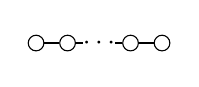
\begin{tikzpicture}[scale=0.4, baseline=-3pt, circ/.style={draw, circle, inner sep=2pt}]
        \node[circ] (1) at (0,0) {}; \node[circ] (2) at (1,0) {}; \node (3) at (2,0) {$\cdots$}; \node[circ] (4) at (3,0) {}; \node[circ] (5) at (4,0) {};
        \draw (1)--(2) (2)--(1.5,0) (2.5,0)--(4) (4)--(5);
    \end{tikzpicture} & $SL_{n+1}, PGL_{n+1}$ \\
    
    % --- Type B ---
    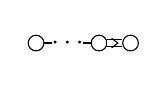
\begin{tikzpicture}[scale=0.4, baseline=-3pt, circ/.style={draw, circle, inner sep=2pt}]
        \node[circ] (1) at (0,0) {}; \node (2) at (1,0) {$\cdots$}; \node[circ] (3) at (2,0) {}; \node[circ] (4) at (3,0) {};
        \draw (1)--(0.5,0) (1.5,0)--(3);
        \draw[double, double distance=2pt] (3) -- (4);
        \draw (2.4,0.15) -- (2.6,0) -- (2.4,-0.15); % Arrow
    \end{tikzpicture} & $SO_{2n+1}$ \\

    % --- Type D ---
    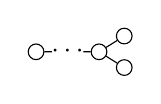
\begin{tikzpicture}[scale=0.4, baseline=-3pt, circ/.style={draw, circle, inner sep=2pt}]
        \node[circ] (1) at (0,0) {}; \node (2) at (1,0) {$\cdots$}; \node[circ] (3) at (2,0) {}; \node[circ] (4) at (2.8,0.5) {}; \node[circ] (5) at (2.8,-0.5) {};
        \draw (1)--(0.5,0) (1.5,0)--(3) (3)--(4) (3)--(5);
    \end{tikzpicture} & $SO_{2n}$ \\

    % --- Type E6 ---
    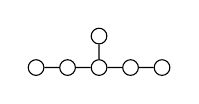
\begin{tikzpicture}[scale=0.4, baseline=-3pt, circ/.style={draw, circle, inner sep=2pt}]
        \node[circ] (1) at (0,0) {}; \node[circ] (2) at (1,0) {}; \node[circ] (3) at (2,0) {}; \node[circ] (4) at (3,0) {}; \node[circ] (5) at (4,0) {}; \node[circ] (6) at (2,1) {};
        \draw (1)--(2)--(3)--(4)--(5) (3)--(6);
    \end{tikzpicture} & $E_6$ \\

    % --- Type G2 ---
    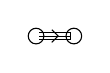
\begin{tikzpicture}[scale=0.4, baseline=-3pt, circ/.style={draw, circle, inner sep=2pt}]
        \node[circ] (1) at (0,0) {}; \node[circ] (2) at (1.2,0) {};
        \draw (1.1,0.1) -- (1.1,-0.1); % Triple line hack or use arrows
        \draw (1.1,0) -- (0.1,0); \draw (1.1,0.1) -- (0.1,0.1); \draw (1.1,-0.1) -- (0.1,-0.1);
        \draw (0.5,0.2) -- (0.7,0) -- (0.5,-0.2); % Arrowhead
    \end{tikzpicture} & $G_2$ \\
\end{tabular}
\fi